%%%%%%%%%%%%%%%%%%%%%%%%%%%%%%%%%%%%%%%%%%%%%%%%%%%%%%%%%%%%
% Document settings
\documentclass{ACGSeminar}

%%%%%%%%%%%%%%%%%%%%%%%%%%%%%%%%%%%%%%%%%%%%%%%%%%%%%%%%%%%%
% Own Packages
\usepackage{amsmath}

%%%%%%%%%%%%%%%%%%%%%%%%%%%%%%%%%%%%%%%%%%%%%%%%%%%%%%%%%%%%
% Own Definitions
\newcommand{\comment}[1]{}


%%%%%%%%%%%%%%%%%%%%%%%%%%%%%%%%%%%%%%%%%%%%%%%%%%%%%%%%%%%%
% BibTex
\bibliography{references}

%%%%%%%%%%%%%%%%%%%%%%%%%%%%%
% Hyphenations here
%%%%%%%%%%%%%%%%%%%%%%%%%%%%%
\hyphenation{Sa-tan-arch-aeo-li-deal-co-hell-ish}


%%%%%%%%%%%%%%%%%%%%%%%%%%%%%
% Title, Author, etc.

\begin{document}

\title{Instant Field-Aligned Meshes}

\author{Til Mohr}


\maketitle

%%%%%%%%%%%%%%%%%%%%%%%%%%%%%%%%%%%%%%%%%%%%%%%%%%%%%%%%%%%%
% Abstract

\begin{abstract}
Remeshing geometries into uniform models is an essential preceding task to many geometry processing algorithms. This paper will examine the instant field-aligned remeshing algorithm presented by Jakob et al. Doing so, this article will first introduce all key concepts used in the algorithm, and will later on present,
how the authors combine these concepts to form their remeshing algorithm. This approach stands out since uses local orientation- and position-fields to compute an isotropic triangular or quad-dominant mesh that is globally aligned with a direction field. Since it accomplishes goals from global remeshing using local optimizations, the method is quite simple complexity-wise and can produce high-quality meshes in no time. To compare to this approach, this paper will also take a closer look at other meshing algorithms and will analyze the performance and quality differences in the resulting meshes.
\end{abstract}

\keywords{remeshing, triangulation, quadrangulation}
\tableofcontents

\newpage

%%%%%%%%%%%%%%%%%%%%%%%%%%%%%%%%%%%%%%%%%%%%%%%%%%%%%%%%%%%%
% Introduction
\label{cha:introduction}
\section{Introduction}
\begin{itemize}
	\item	Why remeshing? $\rightarrow$ Many geometry processing algorithms (smoothing, compression, ...) benefit from isotropic remeshing \cite{surazhsky2003isotropic}. (This is where the paper fits amongst the other papers of the seminar)
\end{itemize}

%%%%%%%%%%%%%%%%%%%%%%%%%%%%%%%%%%%%%%%%%%%%%%%%%%%%%%%%%%%%
% Background
\section{Background}
To fully understand how the algorithm works, we first need to understand some key concepts and techniques. This also helps us to distinguish this approach from other remeshing algorithms.

\subsection{Polygonal meshes}
In computer graphics, there are many possible ways to represent surfaces of digital geometries, such as parametric surfaces, subdivision surfaces, and polygonal meshes. In this paper, we only focus on the latter.\bigskip

A polygonal mesh is a set of polygonal faces, each representing a 2D surface embedded in 3D. Each face consists of a vertex, a 3D point, and edges connecting these vertices. The idea behind polygonal meshes is \textit{cell decomposition}: a complex digital geometry is composed of numerous simple polygonal cells \cite{bommes2013quad}. This allows for performance optimization and reduction of complexity since as an example geometrical formulas on simple polygons are often already predefined. It is very desirable to reduce the number of vertices of each polygonal face to remove complexity. Therefore, polygonal meshes with only very few vertices per face are dominant in computer graphics and geometry processing. The most common categories are triangle meshes and quad meshes. The best type of polygon for a mesh depends on its application.\bigskip

\textbf{Quad meshes} are meshes, where each cell is a quadrilateral. They have a tensor product structure, which is beneficial to many applications such as spline fitting. Because quad meshes have this mathematical benefit, many algorithms are better suited for quad meshes than triangle meshes. Hence they play a major role in computer graphics and geometry processing \cite{bommes2013quad, chen2019quadrilateral}.

Although the quality of a quad mesh isn't specifically defined, there are some indices of a high-quality quad mesh - depending on the application -, such as flat and square faces, and vertices of valency 4. Creating a high-quality pure-quad mesh is a quite challenging task, however. When the geometry's surface has boundaries and curvatures forcing the meshes grid, which is created by square faces, to conform to them, singularities are unavoidable. A \textbf{Singularity} in a mesh is a vertex with irregular valency, a regular valency in a quad mesh, of course, being 4 \cite{fogg2017simple,fogg2018singularities}.

\begin{figure}[htb!]
	\begin{centering}
		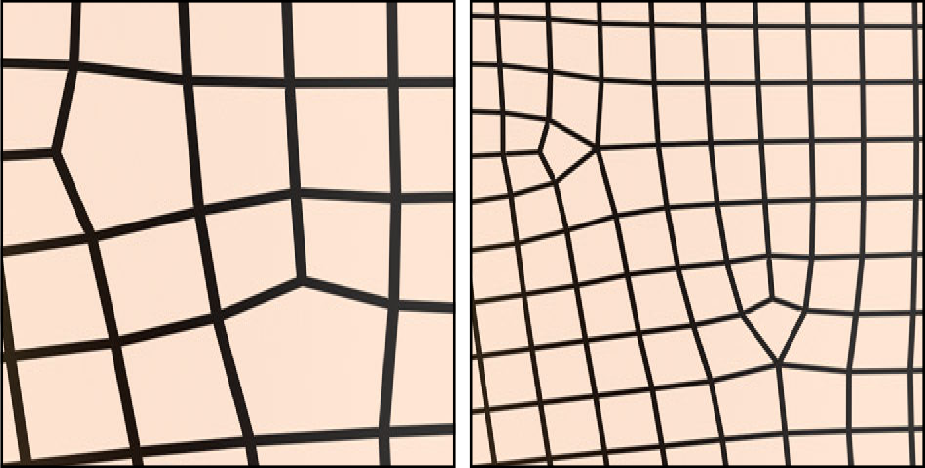
\includegraphics[width=8cm]{img/Singularities.png}\par
	\end{centering}
	\caption{Singularities create pentagons or triangles in quad-dominant mesh \textit{(left)}. Can be transformed into a pure-quad mesh through a subdivision step \textit(right). \cite{jakob2015instant}}
	\label{fig:singularities}
\end{figure}

Because handling these singularities is complicated on its own, oftentimes meshing algorithms resort to quad-dominant meshes. \textbf{Quad-dominant meshes} are meshes, where the majority of faces are quadrilaterals, with some being triangles or pentagons. A quad-dominant mesh can however be converted into a pure-quad mesh through a subdivision step \cite{jakob2015instant}.\bigskip

When a tensor product structure is not needed, often \textbf{triangle meshes} are used because of their simplicity. A benefit here is, that the triangular faces are always flat. As an example, 3D scans produce triangle meshes, although often anisotropic.\bigskip

A mesh is \textbf{isotropic} when it is as "uniform" as possible. This means the faces are of the same size and of the same shape, i.e. equilateral triangles in triangle meshes or squares in quad meshes.


\subsection{Global and local remeshing}
\cite{jakob2015instant,alliez2008recent}
\begin{itemize}
	\item	General inner workings
	\item	Benefits / Disadvantages
		\begin{itemize}
			\item[Global:]	Drastically increased quality
			\item[Local:]	scalability, efficiency, complexity, robustness
		\end{itemize}
\end{itemize}

\subsection{$N$-RoSy fields}\label{rosy}
In geometry a $N$-way rotational symmetry is a property a shape has when it is invariant under rotations of a multiple of $\frac{2\pi}{N}$ around a point or an axis in 2D or 3D respectively \cite{palacios2007rotational}. One can think of these symmetries as vector fields, where each point is associated with $N$ vectors, each pointing in one direction where the symmetry repeats. Hence, we also call these symmetries $N$-way rotational symmetry fields (\textbf{$N$-RoSy fields}) \cite{panozzo2012fields}.

Symmetries also appear on geometrical surfaces, where they are often defined as isometric automorphism. We differ between two categories of symmetries:
\begin{itemize}
	\item	\textbf{Extrinsic} symmetries preserve euclidean distances
	\item	\textbf{Intrinsic} symmetries preserve geodesic distances
\end{itemize}


%%%%%%%%%%%%%%%%%%%%%%%%%%%%%%%%%%%%%%%%%%%%%%%%%%%%%%%%%%%%
% Related Work
\section{Related Work}\label{related_work}
\begin{itemize}
	\item	Previous remeshing approaches from \cite{jakob2015instant}: \cite{ray2006periodic,bommes2009mixed} (since they are also very similar)
	\item	\cite{marcias2015data} to compare to the data driven approach in the seminar
	\item	Focus on type of remeshing (for example local or global, triangle or quad based)
\end{itemize}

%%%%%%%%%%%%%%%%%%%%%%%%%%%%%%%%%%%%%%%%%%%%%%%%%%%%%%%%%%%%
% Main Sections
\section{Method}\label{algorithm}
The following described Instant Field-Aligned Meshes algorithm is a very simple to implement local remeshing approach.

Fundamentally, it takes a graph representation of the geometry's surface as an input and outputs either a triangle-based or a quad-dominant isotropic mesh. To create this mesh, the algorithm computes 2 $N$-RoSy fields (section \ref{rosy}) based on the input graph called orientation- and position-field respectively. In order to align the mesh globally with a direction field, the orientation- and position-field are then optimized iteratively through local smoothing operations - either intrinsically or extrinsically. The output mesh can then be extracted from both fields \cite{jakob2015instant}.

% Input
\subsection{Input representation}
As mentioned, the algorithm takes the geometry's surface represented as an graph $\mathcal{G} = (\mathcal{V}, \mathcal{E})$ for an input. Each element $i \in \mathcal{V}$ is called a vertex and is affiliated with a position $v_i \in \mathbb{R}^3$ and a normal direction $n_i \in \mathbb{R}^3$. $\mathcal{E} \subset \mathcal{V} \times \mathcal{V}$, also called the set of edges, stores neihboring vertices in the graph. Depending on the original geometrical representation, it is defined differently:
\begin{itemize}
	\item	For meshes $\mathcal{E}$ is equal to the usual set of edges in the mesh.
	\item	For point clounds $(i,j) \in \mathcal{E}$, if the vertex $i$ is in the set of $K$-nearest neighbours of $j$.
\end{itemize}

This simple input representation allows for many geometry representations to be used in this algorithm, as long as one can convert it into the described graph format.

% Fields
\subsection{Fields}
FROM 3.1 COMPUTE SMOOTH FIELDS

\subsubsection{Orientation field}
\begin{itemize}
	\item	What for? (why is it important)
	\item	Computation (intrinsic vs extrinsic)
	\item	Singularities
\end{itemize}

\subsubsection{Position field}
\begin{itemize}
	\item	What for? (why is it important)
	\item	Computation (intrinsic vs extrinsic)
	\item	Singularities
\end{itemize}

% Multiresoluion hierarchy
\subsection{Multiresolution hierarchy}
\begin{itemize}
	\item	Problem of local minima
	\item	Solution
\end{itemize}

% Exporting
\subsection{Mesh extraction}
\cite{jakob2015instant}
\begin{itemize}
	\item	Extraction
	\item	(Editing?)
\end{itemize}

%%%%%%%%%%%%%%%%%%%%%%%%%%%%%%%%%%%%%%%%%%%%%%%%%%%%%%%%%%%%
% Results
\section{Results and Discussion}

%%%%%%%%%%%%%%%%%%%%%%%%%%%%%%%%%%%%%%%%%%%%%%%%%%%%%%%%%%%%
% Outlook
%\section{Outlook}

%%%%%%%%%%%%%%%%%%%%%%%%%%%%%%%%%%%%%%%%%%%%%%%%%%%%%%%%%%%%
% Conclusion
\section{Conclusion}
\begin{itemize}
	\item	Quite simple algorithm, but powerful
	\item	Parts can be seperated and used individually (for example you can use the orientation field generation in other algorithms as well)
	\item	Problem of many singularities needs to be dealt with
\end{itemize}

%%%%%%%%%%%%%%%%%%%%%%%%%%%%%%%%%%%%%%%%%%%%%%%%%%%%%%%%%%%%
% Bibliography
\label{cha:references}
\printbibliography

\end{document}
